%!TEX encoding = UTF-8 Unicode
%
% Laboratorio di Fisica III
% Esperienza 11
% Anno accademico 2013/2014
% Daniele Brugnara, Alessandro Casalino
%

\documentclass {article}
\usepackage[utf8]{inputenc}
\usepackage{fontenc}
\usepackage[english]{babel}
\usepackage[%hypertex,
                 unicode=true,
                 plainpages = false, 
                 pdfpagelabels, 
                 bookmarks=true,
                 bookmarksnumbered=true,
                 bookmarksopen=true,
                 breaklinks=true,
                 backref=false,
                 colorlinks=true,
                 linkcolor = blue,		% Use "blue" if you want to highlight them
                 urlcolor  = blue,
                 citecolor = red,
                 anchorcolor = green,
                 hyperindex = true,
                 linktocpage = true,
                 hyperfigures
]{hyperref}
\usepackage{graphicx}
\usepackage{float}
\usepackage{fancyhdr}
\usepackage{listingsutf8}
\usepackage{xcolor}
\graphicspath{{figures/PNG/}{figures/PDF/}{figures/}}
\usepackage{amsfonts}
\usepackage{amsmath}
\usepackage{amssymb}	
\usepackage{wrapfig}
\usepackage{enumitem}
\usepackage{subfigure}
\usepackage{amssymb}
\usepackage{amsmath}
\usepackage [a4paper, top=2.5cm, bottom=2cm, left=1.5cm, right=1.5cm] {geometry}
\pagestyle{fancy}

% cambiato bottom da 1.8 + logo

\makeatletter
\@addtoreset{section}{part}
\makeatother
\rhead{\LARGE Project 1}

\lhead{\large Numerically solving a differential equation}
\lfoot{D. Brugnara, M. Camilli, M. Seclì}
\cfoot{}
\rfoot{\thepage}
\renewcommand{\headrulewidth}{0.7pt}
\renewcommand{\footrulewidth}{0.7pt}

\definecolor{dkgreen}{rgb}{0,0.6,0}
\definecolor{dred}{rgb}{0.545,0,0}
\definecolor{dblue}{rgb}{0,0,0.545}
\definecolor{lgrey}{rgb}{0.9,0.9,0.9}
\definecolor{gray}{rgb}{0.4,0.4,0.4}
\definecolor{darkblue}{rgb}{0.0,0.0,0.6}
\lstdefinelanguage{cpp}{
      backgroundcolor=\color{lgrey},  
      basicstyle=\footnotesize \ttfamily \color{black} \bfseries,   
      breakatwhitespace=false,       
      breaklines=true,               
      captionpos=b,                   
      commentstyle=\color{dkgreen},   
      deletekeywords={...},          
      escapeinside={\%*}{*)},                  
      frame=single,                  
      language=C++,                
      keywordstyle=\color{purple},  
      morekeywords={BRIEFDescriptorConfig,string,TiXmlNode,DetectorDescriptorConfigContainer,istringstream,cerr,exit}, 
      identifierstyle=\color{black},
      stringstyle=\color{blue},      
      numbers=right,                 
      numbersep=5pt,                  
      numberstyle=\tiny\color{black}, 
      rulecolor=\color{black},        
      showspaces=false,               
      showstringspaces=false,        
      showtabs=false,                
      stepnumber=1,                   
      tabsize=5,                     
      title=\lstname,                 
    }

\author{
%\textbf{\normalsize Gruppo A6:}\\
\normalsize Daniele Brugnara \texttt{$<$\href{mailto:daniebru@mail.uio.no}
{daniebru@mail.uio.no}$>$}\\
\normalsize Martina Cammilli \texttt{$<$\href{mailto:martinacam@mail.uio.no}
{martinacam@mail.uio.no}$>$}\\
\normalsize Matteo Seclì \texttt{$<$\href{mailto:mattes@mail.uio.no}
{mattes@mail.uio.no}$>$}
}
\title{\textbf{Project 1: numerically solving a differential equation through a linear system}}

\begin{document}

\maketitle

\hrule
%\medskip
\begin{center}
	\large\textbf{Abstract}
	\medskip\\
	\begin{minipage}[c][][c]{0.8\textwidth}
		\small{
			In this project we aim to solve a special kind of differential equation using a numerical procedure that allows us to express the equation through a linear system. We will study some algorithms to solve such a problem, focusing on the efficiency of the program, setting our goal more on speed than generality.
			}
	\end{minipage}
\end{center}
\medskip
\hrule

\section{Introduction}

The differential equation we're interested in studying is of the type

\begin{equation}
	u''(x)= - f(x)
	\label{differential_eq}
\end{equation}

In our case we will limit our solutions using the contour conditions of $u(0)=0$ and $u(L)=0$, where $[0, L]$ is our domain of integration.
Using Taylor expansion it is possible to express the second derivative of a function $u(x)$ as

\begin{equation}
	u''(x)= \frac{u(x-h)-2 u(x)+u(x+h)}{h^2}+ \O (h^2)
\end{equation}

We are therefore able to discretize equaition (\ref{differential_eq}) using $N$ points, obtaining:

$$u''_i= \frac{u_{i-1}-2 u_i+u_{i+1}}{h^2}=-f_i \quad \quad i \in \left\lbrace 1 \cdots N\right\rbrace$$

Using the matrix representation, we can write equation (\ref{differential_eq}) as

\begin{equation}
 \begin{pmatrix}
   2 & -1 &  0 & 0 & \cdots & 0  \\
  -1 &  2 & -1 & 0 & \cdots & 0  \\
   0 &-1 &  2 & -1 & \cdots & 0 \\
  \vdots  & \vdots  & & \ddots & & \vdots   \\
   0 &  0 & \cdots  & -1 & 2 & -1 \\
   0 &  0 & \cdots & \cdots  & -1 & 2
 \end{pmatrix}
 \begin{pmatrix}
  u_0 \\
  u_1 \\
  u_2 \\
  \vdots  \\
  u_{N-2} \\
  u_{N-1} 
 \end{pmatrix}
 = h^2
 \begin{pmatrix}
  f_0 \\
  f_1 \\
  f_2 \\
  \vdots  \\
  f_{N-2} \\
  f_{N-1} 
 \end{pmatrix}
\end{equation}

Note how, with this system it is already implied that $f(0)=0$ e $f(L)=0$, since the first and last equations state that

$$h^2 f_0=\frac{2 u_0-u_1}{h^2}=\frac{-1 u_{-1}+2 u_0-u_1}{h^2}$$

$$h^2 f_{N-1}=\frac{-u_{N-2}+2 u_{N-1}}{h^2}=\frac{-u_{N-2}+2 u_{N-1}-u_N}{h^2}$$ 

Since the boundary conditions of the differential equations state that $u_{-1}=u(0)=0$ and $u_{N}=u(L)=0$.  

This linear system is indeed very particular and has a clear pattern. We will first focus on finding a solving algorithm for a general tridiagonal matrix and after we will try to implement another program to solve this particular system with the intent of lowering the number of calculation and therefore the computation time.

\section{General algorithm for solving a tridiagonal matrix through back and forward substitution}

A general tridiagonal system can be expressed as

\begin{equation}
 \begin{pmatrix}
   b_0 & c_0 &  0 & 0 & \cdots & 0  \\
  a_1 & b_1 & c_1 & 0 & \cdots & 0  \\
   0 & a_2 &  b_2 & c_2 & \cdots & 0 \\
  \vdots  & \vdots  & & \ddots & & \vdots   \\
   0 &  0 & \cdots  & a_{N-2} & b_{N-2} & c_{N-2} \\
   0 &  0 & \cdots & \cdots  & a_{N-1} & b_{N-1}
 \end{pmatrix}
 \begin{pmatrix}
  u_0 \\
  u_1 \\
  u_2 \\
  \vdots  \\
  u_{N-2} \\
  u_{N-1} 
 \end{pmatrix}
 =h^2
 \begin{pmatrix}
  f_0 \\
  f_1 \\
  f_2 \\
  \vdots  \\
  f_{N-2} \\
  f_{N-1} 
 \end{pmatrix}
\end{equation}

We will describe the algorithm we used for this system first for a 3x3 tridiagonal matrix, and after we will demonstrare its validity for a square tridiagonal matrix of optional dimension.
\\
\\
\\
\\
\\
MATRIX 3X3:

\begin{equation}
\left(
\begin{array}{ccc|c}
   b & c &  0 & f_0 \\
   a & b &  c & f_1 \\
   0 & a &  b & f_2 \\
\end{array}	
\right)
\longrightarrow
\end{equation}
\begin{equation}
Passage 1:
\left(
\begin{array}{ccc|c}
   1 & c/b & 0 & f_0/b \\
   a & b & c & f_1 \\
   0 & a & b & f_2 \\
\end{array}
\right)
\longrightarrow\\
\end{equation}
\begin{equation}
Passage 2:
\left(
\begin{array}{ccc|c}
  1 & c/b & 0 & f_0/b \\
  0 & \frac{b-(c/b)a)}{b-(c/b)a} & \frac{c}{(b-(c/b)a} & \frac{f_1-af_0}{b-(c/b)a} \\
  0 & 0 & \frac{b-\frac{ac}{b-ac/b}}{b-\frac{ac}{b-ac/b}} & \frac{f_2-af_1}{b-\frac{ac}{b-ac/b}} \\ 
\end{array}
\right)
=
\left(
\begin{array}{ccc|c}
  1 & c/b & 0 & f_0/b \\
  0 & 1 & \frac{c}{b-ac/b} & \frac{f_1-af_0}{b-(c/b)a} \\
  0 & 0 & 1 & \frac{f_2-af_1}{b-\frac{ac}{b-ac/b}} \\ 
\end{array}
\right)
\longrightarrow\\\
\end{equation}
\begin{equation}
Passage 3:
\left(
\begin{array}{ccc|c}
  1 & 0 & 0 & f_0/b-f_1(c/b) \\
  0 & 1 & 0 & \frac{f_1-af_0}{b-(c/b)a}-f_2\frac{c}{b-ac/b} \\
  0 & 0 & 1 & \frac{f_2-af_1}{b-\frac{ac}{b-ac/b}} \\
\end{array}
\right)
\end{equation}

Now it's very simple to solve the system.
\\
\\
\\
MATRIX (n+1)x(n+1)

Before starting to demonstrate that the above passages can be done also for a (n+1)x(n+1) matrix, supposed that they work for a nxn one, we can notice that, in general, for a square matrix of optional dimension N, doing the passage 2 until the penultime row we obtain:

$$A_{N-1,N}=\frac{c}{bet(N-1)}$$
where 
$$bet(n)=b_0-\frac{ac}{b_1-\frac{ac}{b_2-\frac{ac}{\frac{\cdots}{b_{n-1}-\frac{ac}{b_n}}}}}$$
(here all the $b_i's$ have the same value; the index i helps only to count them).

Now we do the passage 2 until the last row (we focus only on the tridiagonal matrix; if we manage to obtain the unitary matrix the system is solved); we obtain:

\begin{equation}
\left(
\begin{array}{ccccc}
  1 & c/b & 0 & 0 & \cdots \\
  0 & 1 & fract{c}{b-ac/b} & 0 & \cdots \\
  \cdots & \cdots & \cdots & \cdots & \cdots \\
  \cdots & \cdots & \cdots & 1 & c/bet(n) \\
  \cdots & \cdots & \cdots & 0 & 1 \\
\end{array}
\right)
\end{equation}
and simply subtracting, from the n-row, the (n+1)-row multiplied for bet(n)/c:
\begin{equation}
\left(
\begin{array}{ccccc}
  1 & c/b & 0 & 0 & \cdots \\
  0 & 1 & \frac{c}{b-ac/b} & 0 & \cdots \\
  \cdots & \cdots & \cdots & \cdots & \cdots \\
  \cdots & \cdots & \cdots & 1 & 0 \\
  \cdots & \cdots & \cdots & 0 & 1 \\
\end{array}
\right)
\end{equation}

Now, ignoring the (n+1)-row and the (n+1)-column, we have a nxn matrix which we can bring back to the identity going on with the passage 3.
\\
\\
\\
ALGORITHM IN C++

Translating the above algorithm in C++ language and working only on the vector f and on the solution vector u, we obtain the following code:

\begin{lstlisting}[language=cpp]
	u[0]=f[0]/(bet=b);
    for(int j = 1; j < N; j++) {
        gam[j]=c/bet;
        bet=b-a*gam[j];
        u[j]=(f[j]-a*u[j-1])/bet;
    }
    for (int j = (N-2); j >= 0; j--) u[j] -= gam[j+1]*u[j+1];
\end{lstlisting}
\subsection{Particular algorithm}

Using the regular Gaussian elimination algorithm we proceed to find a specific solution of our system as follows:

\begin{equation}
\left(
\begin{array}{cccccc|c}
   2 & -1 &  0 & 0 & \cdots & 0 & f_0 \\
  -1 &  2 & -1 & 0 & \cdots & 0 & f_1 \\
   0 &-1 &  2 & -1 & \cdots & 0 & f_2\\
  \vdots  & \vdots  & & \ddots & & \vdots & \vdots  \\
   0 &  0 & \cdots  & -1 & 2 & -1 & f_{N-2} \\
   0 &  0 & \cdots & \cdots  & -1 & 2 & f_{N-1} 
\end{array}	
\right)
\longrightarrow
\left(
\begin{array}{cccccc|c}
   2 & -1 &  0 & 0 & \cdots & 0 & f_0 \\
   0 &  3 & -2 & 0 & \cdots & 0 & 2 f_1+f_0 \\
   0 & 0 &  4 & -3 & \cdots & 0 & 3 f_2+2 f_1+f_0\\
  \vdots  & \vdots  & & \ddots & & \vdots & \vdots  \\
   0 &  0 & \cdots  & 0 & N & -(N-1) &  (N-1) f_{N-2} + \sum_{j=0}^{N-3} (j+1)f_{j}  \\
   0 &  0 & \cdots & \cdots  & 0 & N+1 &  \sum_{j=0}^{N-1} (j+1)f_{j} 
\end{array}	
\right)
\end{equation}

We therefore know ahead of times the explicit form of the matrix in upper triangular form and are able to compute all the constant terms of the system as follows

$$\tilde{f}_i= \sum_{j=0}^{i}(j+1) f_j$$

However, we don't need to compute the sum every time, since we can compute $\tilde{f}_i$ knowing $\tilde{f}_{i-1}$:

$$\tilde{f}_i=(i+1)f_i+\tilde{f}_{i-1}$$

Once this forward computations are completed, it is possible to proceed with a back substitution, knowing that

$$u_{N-1}=\frac{1}{N+1} \tilde{f}_{N-1}$$

we are able to find the vector of solutions $u_i$

$$u_i=\frac{1}{i+2} (\tilde{f}[i]+ (i+1) u[i+1])$$

Translating the algorithm in C++ code we obtain the following cycle:

\begin{lstlisting}[language=cpp]
	for (i=1; i!=n; i++) {
		f[i]=(i+1)*f[i]+f[i-1];
	}
	u[n-1]=f[n-1]/(n+1);
	for (i=n-2; i>=0; i--) {
		u[i]=(f[i]+(i+1)*u[i+1])/(i+2);
	}
\end{lstlisting}

Similarly to the previous code of section 1.2 this algorithm is characterized by 2 for cycles and therefore the time required for the solution increase linearly with the number of points used.

Moreover, this program allows us to use a minimal amount of memory, storing only the vector f and the solution u. 


Using the regular Gaussian elimination algorithm we proceed to find a specific solution of our system as follows; we will start form a 3x3 matrix as before, and then demonstrate it for a matrix of optional dimension.
\\
\\
MATRIX 3X3:

\begin{equation}
\left(
\begin{array}{ccc|c}
   2 & -1 & 0 & f_0 \\
   -1 & 2 & -1 & f_1 \\
   0 & -1 & 2 & f_2 \\
\end{array}    
\right)
\longrightarrow
\end{equation}
\begin{equation}
Passage 1:
\left(
\begin{array}{ccc|c}
   2 & -1 & 0 & f_0 \\
   0 & 3 & -2 & f_1(1+1)+f_0 \\
   0 & 0 & 4 & f_2(2+1)+f_1 \\
\end{array}
\right)
\end{equation}
that is: $a_{i,j} \rightarrow (i+1)a_{i,j}+a{i-1,j}$ for i going from 1 to (n-1), where n is the matrix's dimension (3 in this case)
\begin{equation}
\longrightarrow\\
Passage 2:
\left(
\begin{array}{ccc|c}
  2 & -1 & 0 & f_0 \\
  0 & 3 & -1 & f_1(1+1)+f_0 \\
  0 & 0 & 1 & \frac{f_2}{3+1}\\ 
\end{array}
\right)
\end{equation}
that is: $a_{n-1, j} \rightarrow \frac{a{n-1,j}}{n+1}$ where n is the matrix's dimension
\begin{equation}
Passage 3:
\longrightarrow\\
\left(
\begin{array}{ccc|c}
  1 & 0 & 0 & \frac{f_0+(0+1)f_1}{0+2} \\
  0 & 1 & 0 & \frac{f_1+(1+1)f_2}{1+2} \\
  0 & 0 & 1 & \frac{f_2}{3+1} \\
\end{array}
\right)
\end{equation}
that is $a_{i,j} \rightarrow \frac{a_{i,j}+(i+1)a_{i+1,j}}{i+2}$ for i going from 0 to (n-1)
\\
Now it's very simple to solve the system.
\\
\\
\\
MATRIX (n+1)x(n+1)

We focus only on the tridiagonal matrix and try to obtain the unitary matrix; to do this let's to passage 1 until the n+1 row.

\begin{equation}
\left(
\begin{array}{ccccc}
  2 & -1 & 0 & 0 & \cdots \\
  0 & 3 & -2 & 0 & \cdots \\
  \cdots & \cdots & \cdots & \cdots & \cdots \\
  \cdots & \cdots & \cdots & n+2 & -(n+1) \\
  \cdots & \cdots & \cdots & 0 & n+3 \\
\end{array}
\right)
\end{equation}
Now let's do passage 2 on the n+1 row
\begin{equation}
\left(
\begin{array}{ccccc}
  2 & -1 & 0 & 0 & \cdots \\
  0 & 3 & -2 & 0 & \cdots \\
  \cdots & \cdots & \cdots & \cdots & \cdots \\
  \cdots & \cdots & \cdots & n+2 & -(n+1) \\
  \cdots & \cdots & \cdots & 0 & n+3 \\
\end{array}
\right)
\end{equation}

Now, ignoring the (n+1)-row and the (n+1)-column, we have a nxn matrix which we can bring back to the identity going on with the passage 3.
\\
\\
\\
ALGORITHM IN C++

Translating the above algorithm in C++ language and working only on the vector f and on the solution vector u, we obtain the following code (N is the matrix's dimension):

\begin{lstlisting}[language=cpp]
    for(int j = 1; j < N; j++) f[j]=(j+1)*f[j]+f[j-1];
    u[N-1] = f[N-1]/(N+1);
    int prev_idx = N;
    for(int j = N - 1; j > 0; j--) {u[j-1]=(f[j-1]+j*u[j])/prev_idx; prev_idx = j;}
\end{lstlisting}





\section{Errors}
It is now interesting to analyse the error that we do in numerical approximation as a function of the number of points. It is intuitive that, as much as we restrict the step length $h$ (that is the same thing as increasing the number of points) the error gets smaller and smaller. This behaviour is shown if Figure \ref{fig:errors}, where we plotted in a log-log scale the maximum percentage error calculated as
\begin{equation*}
	\epsilon_i = \left| \frac{v[i]}{u[i]} - 1 \right|
\end{equation*}
($v[i]$ is the numerical solution, $u[i]$ is the analytical one).
\begin{figure}[H]
	\centering
	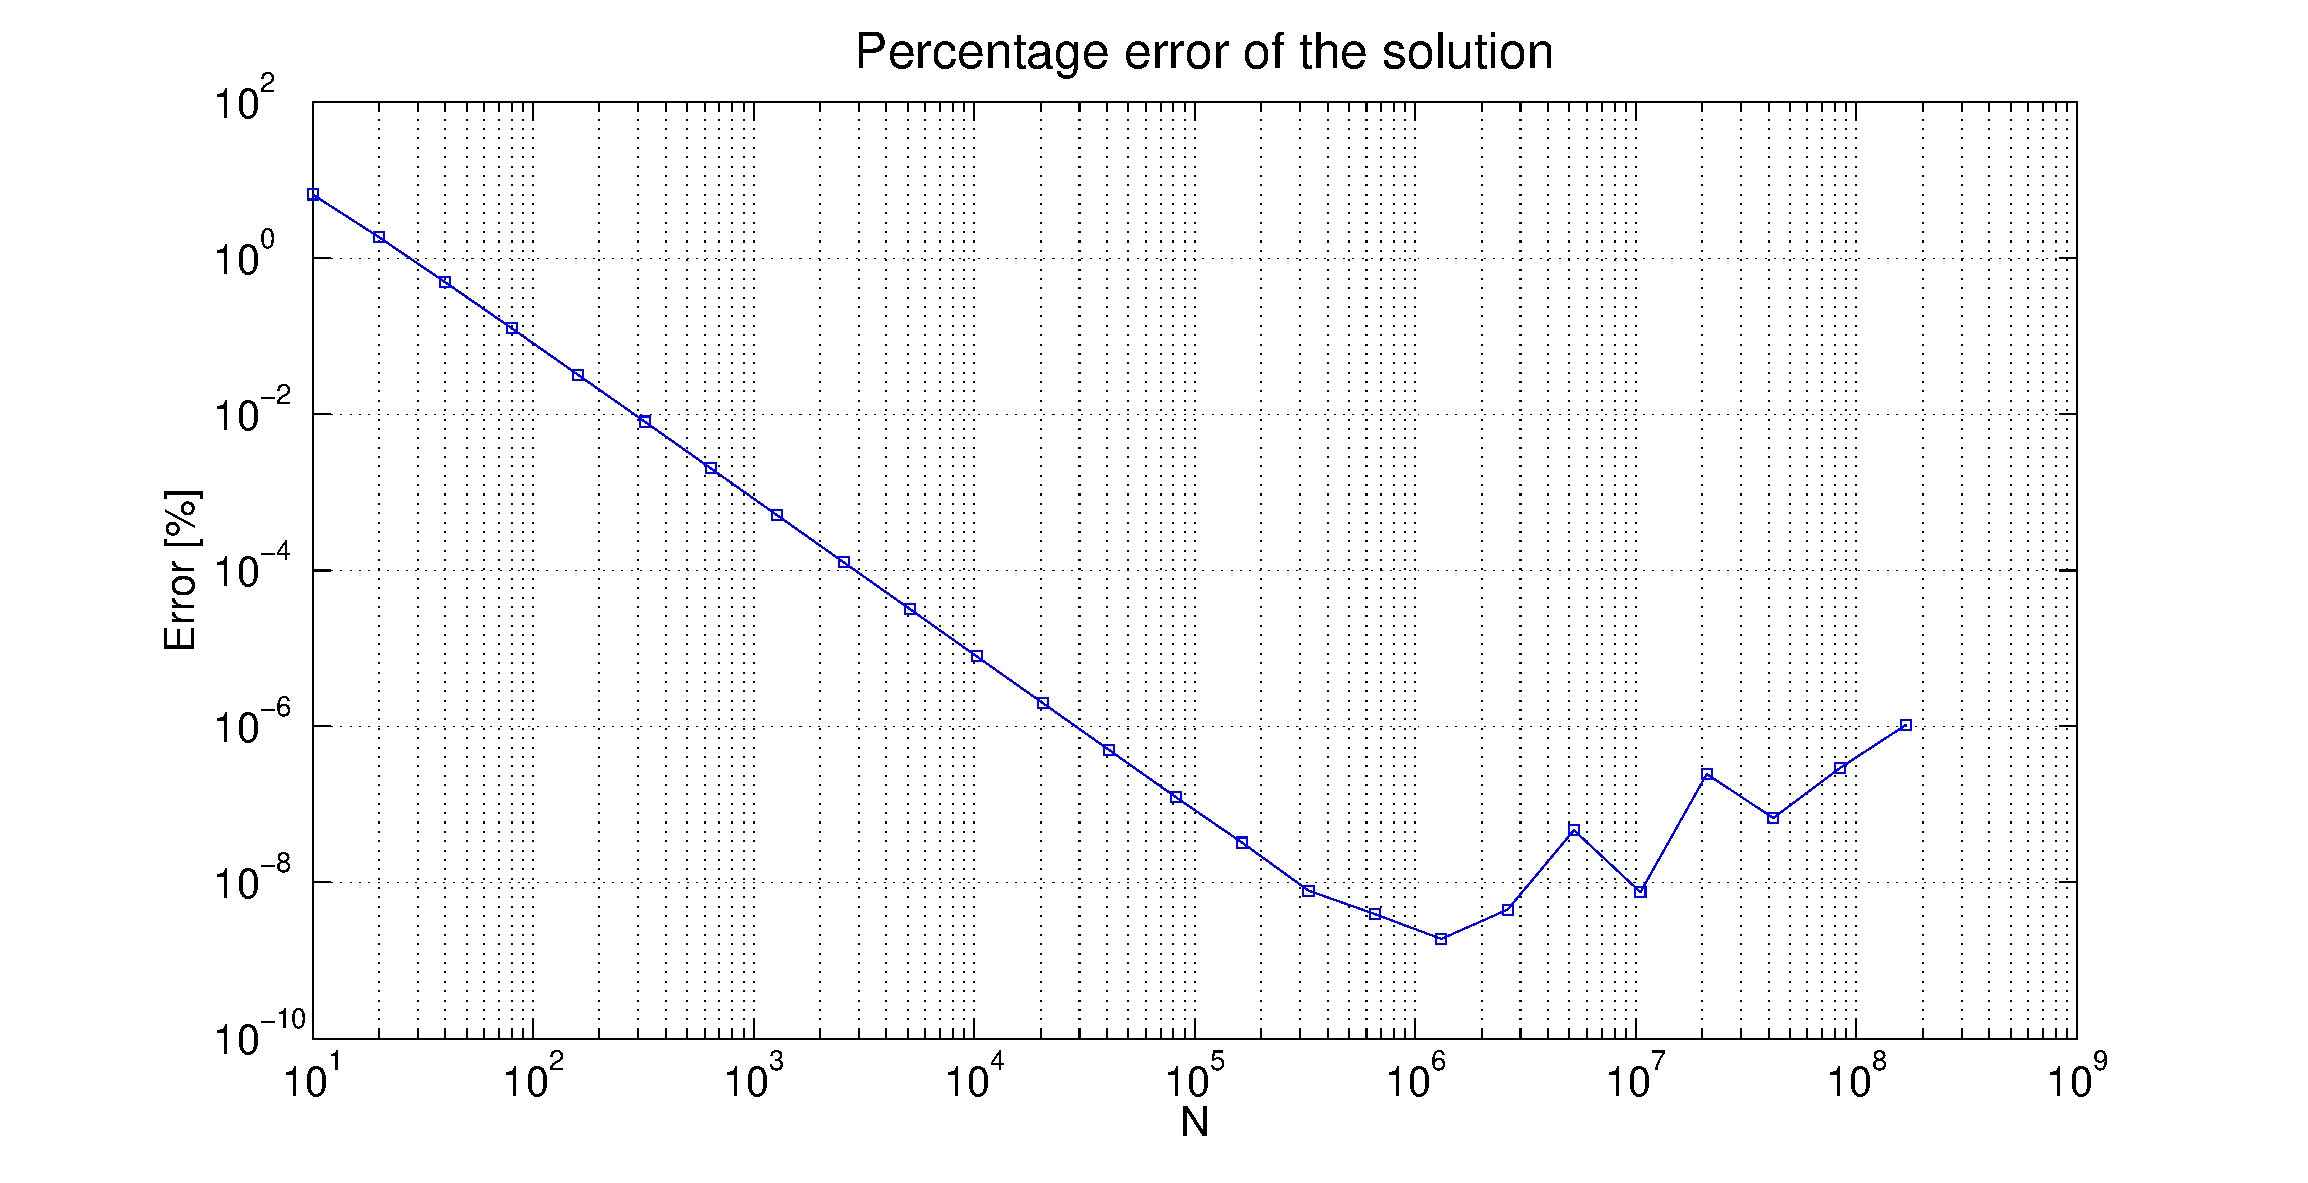
\includegraphics[width=\textwidth]{errors}
	\caption{Maximum percentage error of the numerical solution as a function of the number of points.}
	\label{fig:errors}
\end{figure} 
You see that the error lowers until $N = 10^{5}$, then increases again. This a typical example of \emph{loss of precision}; as our numerical solution gets closer to the analytical one, the ratio $v[i]/u[i]$ gets closer to one, and as a result in calculating $\epsilon_i$ we perform a subtraction between two almost identical (in our choice of precision) numbers. This causes a loss in terms of significant digits that explains the behaviour of the plot for big $N$. It is also evident that we get the lowest significant relative error for $N \simeq 10^{6}$. Relative errors for $N > 10^{6}$ are not worth trusting, due to the loss of precision explained above.




\section{Time}

We will now study how the program performs as a function of the dimension of the matrix. 

\begin{figure}[ht]
 \centering
   {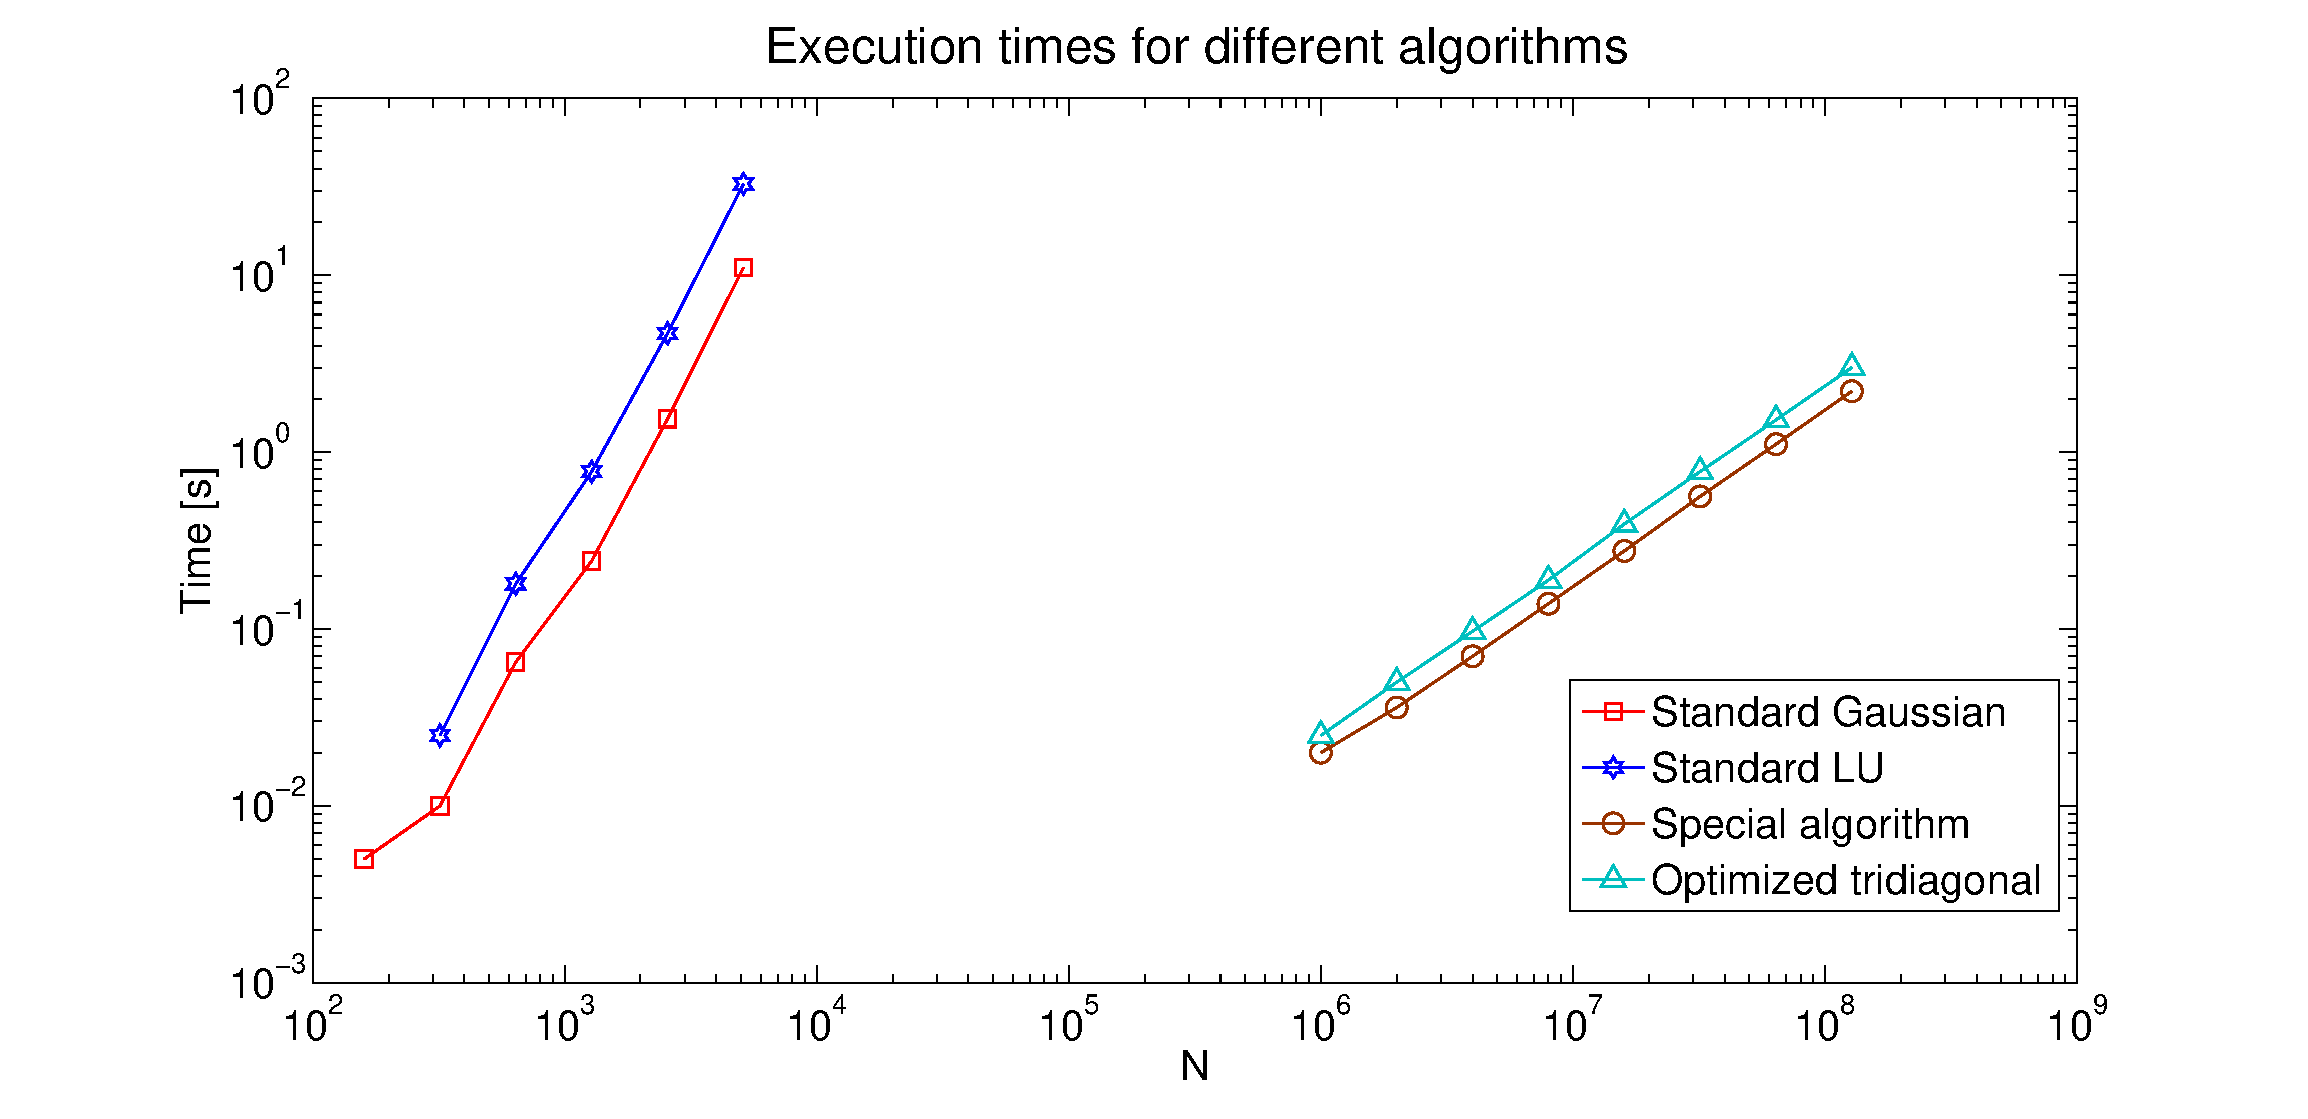
\includegraphics[width=18cm]{times.eps}}
 \caption{Elapsed time during calculation for the various algorithms on a logarithmic grid.}
\end{figure}

In Figure (1) we can notice how a specialized algorithm is indeed able to significantly cut down the time required for the computation of the solution.
In fact, we can easily notice how, with a standard Gaussian elimination, the required time for solving a $2 \times 10^2$  dimensional matrix is the same it takes for the specialized algorithm to compute $10^6$ points. This yields clearly to a much higher degree of precision and a better deployment of resources.
As a matter of fact, counting the number of operations contained in the for cycle for the specialised algorithm is 


\newpage
\section{C++ Code}

\begin{lstlisting} [language=cpp]
#include <iostream>
#include <fstream>
#include <armadillo>
#include <cstdlib>
#include <cmath>
#include <ctime>
using namespace std;
using namespace arma;
namespace use {int onealg = 0; int out = 1;}
// 'fill_matrix' fills the matrix A in a tridiagonal form.
void fill_matrix(mat& A, int N) {
//Fill the matrix
A(0,0) = 2;
A(0,1) = -1;
for(int i = 1; i < N-1; i++){
A(i,i-1) = -1;
A(i,i) = 2;
A(i,i+1) = -1;
}
A(N-1,N-2) = -1;
A(N-1,N-1) = 2;
}
// 'solve_gaus' solves the system with a standard gaussian decomposition
void solve_gaus(vec& u, vec& f, int N){
//Start timing
clock_t t;
t = clock();
//Define our matrix and initialize it
mat A(N,N);
A.zeros();
fill_matrix(A,N);
//Just the decomposition
u = solve(A,f);
A.reset();
//Stop timing
t = clock() - t;
cout <<"Elapsed time (solve_gaus):\t\t" <<((float)t)/CLOCKS_PER_SEC <<"s." <<endl;
}
// 'solve_lu' solves the system with a standard LU decomposition
void solve_lu(vec& u, vec& f, int N){
//Start timing
clock_t t;
t = clock();
//Define our matrix and initialize it
mat A(N,N);
A.zeros();
fill_matrix(A,N);
//Define workspace matrices
mat L(N,N), U(N,N), P(N,N);
//Do the decomposition
lu(L, U, P, A);
A.reset();
//Just solve the system
vec b;
b = solve(L,P*f);
L.reset();
P.reset();
u = solve(U,b);
U.reset();
//Stop timing
t = clock() - t;
cout <<"Elapsed time (solve_lu):\t\t" <<((float)t)/CLOCKS_PER_SEC <<"s." <<endl;
}
// 'solvetrid' is a function that solves a linear sistem in 'u' relative to a
// tridiagonal matrix with diagonal elements equal to 'b', subdiagonal elements
// equal to 'a' and superdiagonal elements equal to 'c'. Returns the result
// in the vector 'u', overwriting its elements. The algorithm performs ~8N FLOPS.
void solvetrid(int& N, float& a, float& b, float& c, vec& u, vec& f){
// Start timing
clock_t t;
t = clock();
// Define the variable 'bet', that is just the denominator of 'gam',
// and 'gam' itself, that is a workspace vector
double bet;
vec gam(N);
// Start forward substitution
u[0]=f[0]/(bet=b);
for(int j = 1; j < N; j++) {
gam[j]=c/bet;
bet=b-a*gam[j];
u[j]=(f[j]-a*u[j-1])/bet;
}
// Just one-line backward substitution
for (int j = (N-2); j >= 0; j--) u[j] -= gam[j+1]*u[j+1];
// Stop timing and print elapsed time
t = clock() - t;
cout << "Elapsed time (solvetrid):\t\t" << ((float)t)/CLOCKS_PER_SEC << "s." << endl;
// Free space
gam.reset();
}
// 'solve_special' is a function that solves a special linear system
// relative to a tridiagonal matrix with b = 2 and a = c = -1. The
// solution has been found analytically, and once the pattern in
// the solution was recognized, it has been coded here. Warning! It
// overwrites 'u' and 'f', so make a copy before calling the function
// if you want to re-use them. The alogrithm performs ~6N FLOPS.
void solve_special(int& N, vec& u, vec& f){
// Start timing
clock_t t;
t = clock();
for(int j = 1; j < N; j++) f[j]=(j+1)*f[j]+f[j-1];
u[N-1] = f[N-1]/(N+1);
int prev_idx = N;
for(int j = N - 1; j > 0; j--) {u[j-1]=(f[j-1]+j*u[j])/prev_idx; prev_idx = j;}
// Stop timing and print elapsed time
t = clock() - t;
cout << "Elapsed time (solve_special):\t\t" << ((float)t)/CLOCKS_PER_SEC << "s." << endl;
}
// 'split' is a function that discretizes the function 'func',
// storing its values in N points from 0 to 1 in the vector 'f'.
// Grid points are stored in the vector 'x'.
void split(vec& f, vec& x, int& N) {
// Define points spacing and calculate the grid points
// and the value of func in those points
double h = 1.0/(N+1);
double h_square = pow(h,2);
for(int i = 0; i < N; i++){
x[i] = (i+1)*h;
f[i] = h_square*100*exp(-10*x[i]);
}
}
// 'relative_error' calculates the relative error with respect to the
// theoretical value 'u_th(x)'.
vec relative_error(vec& u, vec& x, int& N) {
vec err(N);
err[0] = 0;
for(int i = 0; i <= N-1; i++){
err[i] = abs( u[i]/(1-(1-exp(-10))*x[i]-exp(-10*x[i])) - 1 );
}
return err;
}
// 'main' takes as first argumt the number of points that the program
// will use during the calculation. Use 'onealg 1' as second argument
// if you want to use only one algorithm and write to the output file.
// Use 'anealg 0' if you want to use only one algorithm and don't write
// to the output file.
int main(int argc, char *argv[])
{
int N = atoi(argv[1]);
// Perform some checks in the optional argument.
if(argc == 4) {
use::out = atoi(argv[3]);
if(strcmp(argv[2], "onealg") == 0 && (strcmp(argv[3], "1") == 0||strcmp(argv[3], "0") == 0)) use::onealg = 1;
else cout << "Wrong optional argument given. Use 'onealg 1' if you want to use only one algorithm (the fastest) and write to file; use 'onealg 0' if you instead want to write to the output file." << endl;
}
// Define the elements of the matrix related to the differential equation
float a = -1.0;
float b = 2.0;
float c = -1.0;
// Initialize the solution vector 'u' with zeros and the vector 'f'
// of the function values
vec u = zeros<vec>(N);
vec f(N), x(N);
//for(int i = 0; i < N; i++) f[i] = i+1;
// Discretize and define workspace vectors
split(f, x, N);
vec u_temp(N), f_temp(N), err(N);
// Compare algorithms only if we want to do benchmarks.
// This is to save memory if we want just to have grid numbers.
if(use::onealg == 0) {
// Solve using 'solve_lu' and 'solve_gaus'
if (N <= 10000) {
solve_lu(u,f,N);
solve_gaus(u,f,N);
}
// Solve using 'tridig'
solvetrid(N, a, b, c, u, f);
}
// Solve using 'solve_special'
solve_special(N, u, f);
f.reset();
// Compute relative error only if 'onealg' is enabled, to speed up benchmarks
if(use::onealg == 1) {
err = relative_error(u, x, N);
cout << "Maximum relative error: " << err.max()*100 << "%" << endl;
}
// Write the resulting points on the output file
if(use::onealg == 1 && use::out == 1) {
// Write the 'x' grid-points to the output file
ofstream X;
X.open("X.txt");
X << x;
X.close();
// Write the 'u' grid-points to the output file
ofstream U;
U.open("U.txt");
U << u;
U.close();
// Write the error bars to the output file
ofstream E;
E.open("E.txt");
E << err;
E.close();
}
return 0;
}
\end{lstlisting}

\end{document}